% ------------------------------------------------------------------
\renewcommand{\thisunit}{MATH327 Unit 10}
\renewcommand{\moddate}{Last modified 12 May 2023}
\setcounter{section}{10}
\setcounter{subsection}{0}
\phantomsection
\addcontentsline{toc}{section}{Unit 10: Synthesis and broader applications}
\section*{Unit 10: Synthesis and broader applications} % TODO: Synthesizing interacting systems with numerical techniques used for computer project...
\subsection{\label{sec:MonteCarlo}Monte Carlo importance sampling}
Although we were able to derive some exact results for the Ising model in one and two dimensions, it's worth recalling that for $3 \leq d < \infty$ no exact solution is known even for this simple system.
In general, interacting statistical systems are not exactly solvable.
In order to explore their broad applications throughout the mathematical sciences and beyond, we therefore need to analyze them either through systematic approximation schemes (such as \emph{perturbation theory}) or by numerical computations.
Numerical methods have become increasingly important over the past fifty years, and in this section we'll outline the general methods they employ.

Our goal is to compute expectation values of interest, which are formally defined by sums over all micro-states.
Considering the canonical ensemble for simplicity,
\begin{equation*}
  \vev{\cO} = \sum_{i = 1}^M \cO_i \; p_i = \frac{1}{Z} \sum_{i = 1}^M \cO_i \; e^{-\be E_i} = \frac{\sum_{i = 1}^M \cO_i \; e^{-\be E_i}}{\sum_{i = 1}^M e^{-\be E_i}}.
\end{equation*}
We already saw, at the end of \secref{sec:Ising}, that enormous computational resources would be required to carry out such sums over micro-states.
Even for tiny Ising systems with $N \sim 1000$ spins, the largest existing or foreseeable supercomputers would have to run for far longer than the age of the universe in order to evaluate the roughly $2^{1000} \sim 10^{300}$ terms in the partition function.
To quantify `tiny', consider that $N \sim 1000$ would correspond to a $10\times 10\times 10$ lattice in three dimensions or a $6\times 6\times 6\times 6$ lattice in four dimensions, both very far from the $N \to \infty$ thermodynamic limit of interest for phase transitions.

And yet, at the end of \secref{sec:mean_field} we were able to quote numerical results for the Ising model critical temperature for $3 \leq d \leq 7$, along with a $d = 3$ critical exponent.
These results are obtainable because practical numerical computations do not perform a `brute-force' evaluation of every single micro-state.
Instead, they proceed by (pseudo-)randomly \textbf{sampling} a very small subset of those micro-states, and using this subset to compute results for the average energy, magnetization, and other thermodynamic quantities.
So long as this sampling is done appropriately, the law of large numbers allows us to treat these averages as controlled approximations to the true ensemble expectation values.

As we saw in the computer project, such numerical calculations employ pseudo-random numbers rather than complete randomness, which allows them to be reproducible up to very high precision by different people using different computers.
Due to the role of randomness, these numerical approaches have become known as \textbf{Monte Carlo} methods, based on a whimsical reference to the famous gambling centre in Monaco.
Monte Carlo methods are crucial in statistical physics, and related disciplines, because they are very broadly applicable to interacting systems that no longer benefit from dramatic simplifications through factorization.

We can gain some intuition about how Monte Carlo methods work by using such pseudo-random sampling to numerically evaluate a simple integral.
The idea is that the integral can be numerically approximated by evaluating its integrand at randomly sampled points in the integration domain, and normalizing by the number of samples.
An amusing example is to compute
\begin{align*}
  \pi & = \int_{-1}^1 dx \int_{-1}^1 dy \ H\!\left(1 - \left\{x^2 + y^2\right\}\right) \qquad &
  H(r) & = \left\{\begin{array}{l}1 \qquad \mbox{for } \ r \geq 0 \\
                                  0 \qquad \mbox{for } \ r < 0\end{array}\right. ,
\end{align*}
where the Heaviside step function $H(r)$ picks out a disk with radius $R = 1$ in a square integration domain with area $4$, as shown below.
Since the integrand is either $0$ or $1$ for each randomly sampled point in that domain, simply counting the fraction of the $S$ samples that lie in the disk provides a numerical determination of $\pi$, with a \textit{statistical uncertainty} that vanishes $\propto 1 / \sqrt{S}$.
In just a few minutes, \href{https://github.com/daschaich/MATH327_2023/blob/main/lecture_notes/unit10_pi.py}{this Python code} predicts $\pi = 3.14152 \pm 0.00023$ purely from sampling pseudo-random numbers.

\begin{center}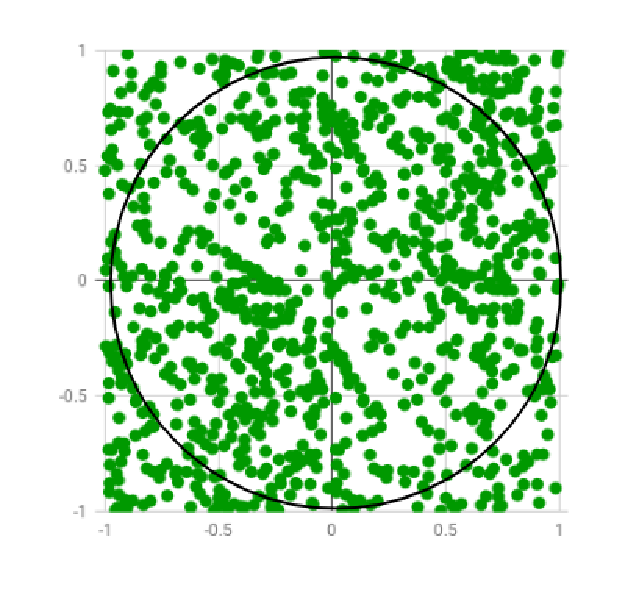
\includegraphics[width=0.6\textwidth]{figs/unit10_pi.pdf}\end{center}

Of course, numerically computing $\pi$ can be done far more efficiently with other, more specialized, techniques.
Monte Carlo integration is most useful when we need to consider very high-dimensional integrals --- such as partition functions of interacting statistical systems, interpreted as $N$-dimensional integrals over the system's $N$ degrees of freedom.
To illustrate the scale of computations that can currently be carried out, ongoing theoretical physics research here in Liverpool routinely uses Monte Carlo methods to numerically evaluate roughly billion-dimensional integrals.

At this point, you might be concerned that such sampling can account for only an extremely small fraction of the possible micro-states for the systems under consideration, suggesting a risk of inaccurate results from unrepresentative sampling.
This is a new manifestation of the obstacle we encountered when considering brute-force computations above.
If the brute-force evaluation of every single micro-state takes far longer than the age of the universe, then the fraction we could sample in a reasonable amount of time (say, a day) is almost vanishingly small.

As a concrete example, if we generously suppose our computer only needs a few nanoseconds to sample a micro-state of a tiny $N \sim 1000$ Ising system, over the course of a day it would sample roughly ten trillion ($10^{13}$) spin configurations --- only about one part in $10^{287}$ of the total $2^N \sim 10^{300}$ micro-states.
To make the situation even worse, as $N$ increases the number of possible Ising model micro-states grows \textit{exponentially} quickly, $\sim$$2^N$, in addition to the more modest growth in the amount of computing required to sample each micro-state.
For illustration, 2015 research \href{https://arxiv.org/abs/1502.07613}{arXiv:1502.07613} numerically predicting $T_c$ for the Ising model in $d = 5$, $6$ and $7$ dimensions includes calculations up to $N = 64^5 \approx 10^9$.
Out of the roughly $2^{10^9} \sim 10^{323{,}000{,}000}$ micro-states for this systems, only $\sim$$10^4$ could be sampled in a reasonable amount of time.
How much trust should we place in results from such numerical work?

Thinking back to our consideration of the ordered and disordered phases of the Ising model in \secref{sec:Ising_phases}, we could make a case that everything may work out in the high-temperature disordered phase.
In the infinite-temperature limit, all the micro-states become equally probable, and observable expectation values are determined by the degeneracies of the different energy levels.
Random sampling is more likely to account for the dominant energy levels with large degeneracies, making it plausible that reasonable results could be obtained by averaging even over such a tiny fraction of the total number of micro-states.

In the low-temperature ordered phase, however, the opposite occurs.
As the temperature decreases, the large-scale behaviour of the system in this phase is dominated by a very small number of micro-states.
For sufficiently low temperatures, observable expectation values are effectively determined by the two degenerate minimum-energy micro-states with all spins aligned either up or down.
Only exponentially suppressed corrections would then be introduced by higher-energy excited states.
As there is essentially no chance of randomly sampling either of those two minimum-energy micro-states, the random sampling approach described above seems doomed to fail.

A key breakthrough that made numerical results truly reliable was the invention of stochastic procedures to sample any micro-state $\om_i$ with a probability proportional to its Boltzmann factor, $p_i \propto e^{-\be E_i}$.
Such automated procedures are known as \textit{algorithms} (a term that evolved from the name of \href{https://en.wikipedia.org/wiki/Muhammad_ibn_Musa_al-Khwarizmi}{Muhammad ibn Musa al-Khwarizmi}), and the overall approach is called \textbf{importance sampling}, since it preferentially samples the important micro-states that make the most significant contributions to the partition function and derived quantities. % TODO: Persian mathematician active in the early 9th century...
Assuming we have such an algorithm, applying it to the $\be \to \infty$ low-temperature phase considered above would produce an exponentially enhanced probability of sampling low-energy micro-states, as desired.
As $\be \to 0$ in the high-temperature phase, there would be little change compared to the more straightforward pseudo-random sampling considered above, since all micro-states would become equally probable.

The challenge is to design importance sampling algorithms in the first place.
In particular, these algorithms can't rely on knowing the full set of micro-state energies $E_i$, and the corresponding probabilities $p_i$, since enumerating these data would be equivalent to brute-force computation of the full partition function.
In essence, the algorithm has to exploit its stochastic aspect --- its use of pseudo-random numbers --- to guide it to important, high-probability micro-states.
And this guiding needs to be done without introducing any other bias that might cause distorted results to be obtained from averaging over the tiny fraction of micro-states that can be sampled in a reasonable amount of time.

A \href{https://en.wikipedia.org/wiki/Equation_of_State_Calculations_by_Fast_Computing_Machines}{famous solution} to this challenge was developed in 1953 by \href{https://en.wikipedia.org/wiki/Nicholas_Metropolis}{Nick Metropolis}, \href{https://en.wikipedia.org/wiki/Arianna_W._Rosenbluth}{Arianna Rosenbluth}, \href{https://en.wikipedia.org/wiki/Marshall_Rosenbluth}{Marshall Rosenbluth}, \href{https://en.wikipedia.org/wiki/Augusta_H._Teller}{Mici Teller} and \href{https://en.wikipedia.org/wiki/Edward_Teller}{Edward Teller}.
I will call this solution the Metropolis--Rosenbluth--Teller algorithm, or the MRT algorithm for short.\footnote{In an infamous misfiring of alphabetical ordering, this remains widely known as the ``Metropolis algorithm'' even though Metropolis's role was providing specialized computing equipment rather than creating the algorithm itself.  In addition, the key contributions of Arianna Rosenbluth and Mici Teller were widely under-appreciated for many years.}
It relies on the concept of Markov chains that we briefly discussed when considering random walks all the way back in \secref{sec:diffusion}.
To reiterate the key concept, a Markov chain is a process in which the next micro-state to be sampled is pseudo-randomly chosen based on the micro-state currently under consideration, with no `memory' of any other micro-states that may previously have been sampled.

We can use the Ising model to illustrate how the MRT algorithm employs Markov chains to sample micro-states proportionally to their importance.
Any spin configuration can serve equally well as the initial micro-state at the start of the chain.
Starting from this initial configuration, we pseudo-randomly select one spin, $s_j$, and compute $\De E_j$, the change in the system's energy that would be caused by flipping $s_j \to -s_j$.
We then update the spin configuration by `accepting' this spin flip with probability
\begin{equation}
  \label{eq:MRTprob}
  P_{\text{accept}} = \mbox{min}\left\{1, e^{-\be \De E_j}\right\},
\end{equation}
which defines the next micro-state in the Markov chain.
Importantly, this new micro-state may be identical to the previous micro-state --- this occurs with probability $P_{\text{reject}} = 1 - P_{\text{accept}}$.
The final step of the algorithm is to repeat this single-spin update procedure as many times as our computers can handle.

We can appreciate why micro-states may need to be repeated in the Markov chain by considering what should happen if we were to sample the ground state at low temperatures.
In this regime, the ground state should dominate, so the algorithm should sample it repeatedly, proportionally to its probability.

Digging into \eq{eq:MRTprob}, we can see that any spin flip that lowers the energy will always be accepted, since $\De E < 0 \implies e^{-\be \De E} > 1$.
The MRT algorithm is therefore free to approach the minimum-energy ground state of the system.
If it is in the ground state, then any spin flip will increase the energy, $\De E > 0$, and will only be accepted with an exponentially suppressed probability $e^{-\be \De E} \to 0$ as $T = 1 / \be \to 0$, as desired.
More generally, if we consider two micro-states $\om_A$ and $\om_B$, then the relative probabilities of moving between these two micro-states are
\begin{equation}
  \label{eq:MRTdistribution}
  \frac{P(A \to B)}{P(B \to A)} = \frac{\mbox{min}\left\{1, e^{-\be(E_B - E_A)}\right\}}{\mbox{min}\left\{1, e^{-\be(E_A - E_B)}\right\}} = \frac{e^{-\be(E_B - E_A)}}{1} = \frac{e^{-\be E_B}}{e^{-\be E_A}},
\end{equation}
regardless of whether $E_A \leq E_B$ or $E_B \leq E_A$.

So long as every micro-state can be generated from any other micro-state by making a series of pseudo-random changes to individual degrees of freedom, \eq{eq:MRTdistribution} ensures that the micro-states $\om_i$ will indeed be sampled with probabilities proportional to the Boltzmann factors $e^{-\be E_i}$ that quantify their importance.
The necessary condition that the Markov chain can reach every micro-state (at least in principle) is called \textbf{ergodicity}.
Because the micro-state probabilities $p_i$ are effectively `felt out' through the accept/reject test described above, in non-ergodic situations the algorithm will fail to account for the probabilities of micro-states that can't be reached by the Markov chain.
This can easily lead to incorrect results.

You can read more about the MRT algorithm in Section~8.2 of Dan Schroe-der's \textit{Introduction to Thermal Physics} (the second item in the list of further reading on page~5), which provides a single-page annotated code implementing it for the two-dimensional Ising model. % WARNING: Hyphenating by hand
While the conceptually simple MRT algorithm is the most famous means to carry out Markov-chain Monte Carlo importance sampling, it is far from the only option, and often far from the best.
If time permits, we may discuss some of the challenges that make it advantageous to go beyond the MRT algorithm, in particular the issue of \textbf{auto-correlations}.

For now, suffice it to say that there is an enormous amount of ongoing research developing, optimizing and applying more elaborate Monte Carlo methods to investigate topics throughout the mathematical sciences and beyond.
In \secref{sec:broad} we will briefly look at some of these broader applications.
First, there is another important concept to introduce, called universality, which helps to reveal why interacting statistical systems are so useful to apply to such a diverse range of scientific investigations.
% ------------------------------------------------------------------



% ------------------------------------------------------------------
\subsection{Universality}
In \secref{sec:mean_field} we defined the critical exponent $b$ as the non-integer power governing the behaviour of the order parameter $\vev{m} \propto \left(T_c - T\right)^b$ for temperatures slightly lower than the critical temperature $T_c$ of the second-order phase transition.
In addition to being an important characteristic any specific phase transition, it was discovered during the twentieth century that precisely the same critical exponents turn out to govern the behaviour of phase transitions that we initially would not have expected to have any connection.

A famous example of universality involves the \textbf{liquid--gas phase transition}, which we have run out of time to discuss in detail.
This phase transition occurs only for interacting (non-ideal) gases, and after our studies of simple interacting spin systems in Unit~9 we can appreciate that such interacting gases are far more difficult to analyze than the ideal gases we considered in Units~4 and 8.
Section~8.2 of Dan Schroeder's \textit{Introduction to Thermal Physics} explains some tricks that can simplify these calculations in certain regimes.
Specifically, the equation of state of a low-density interacting gas can be expressed as an expansion around the ideal gas law,
\begin{equation*}
  PV = NT\left[1 + B(T) \rho_{\text{gas}} + \cO\left(\rho_{\text{gas}}^2\right)\right],
\end{equation*}
where $\rho_{\text{gas}}$ is the density of the atoms in the gas, which needs to be small in order for this approach to work.
The temperature-dependent function that governs the leading correction to the ideal gas law,
\begin{equation*}
  B(T) = -2\pi \int_0^{\infty} r^2 \left(e^{-u(r) / T} - 1\right) \; dr,
\end{equation*}
in turn depends on the interaction energy $u(r)$ between pairs of particles separated by distance $r$, which can vary significantly for different types of particles.

Unfortunately, the restriction to low densities in this analysis prevents its application to the liquid--gas phase transition.
From everyday experience we can appreciate that the liquid phase of a given set of particles (for example, water) has a higher density than the gas phase of those same particles (in this case, steam).
The liquid--gas phase transition occurs at the critical temperature $T_c$ that produces equal densities for the two phases --- this is the largest density the gas can reach while still remaining a gas, rather than the low density assumed above.

An alternative approach, pioneered by \href{https://en.wikipedia.org/wiki/Johannes_Diderik_van_der_Waals}{Johannes van der Waals} in the late 1800s (and awarded the 1910 Nobel Prize in Physics), is to propose modifications to the equation of state based on qualitative physical arguments.
The van der Waals equation of state,
\begin{equation*}
  \left(P + a\rho^2\right)\left(V - Nb\right) = NT,
\end{equation*}
aims to model two aspects of interacting fluids and gases, through two unknown parameters $a$ and $b$.
First, $Nb$ represents the non-zero volume occupied by the $N$ particles, which is subtracted from the total available volume $V$.
Second, the $a\rho^2$ dependence on the density represents repulsive forces that the particles exert on each other when they are packed more closely together.

These are obviously rough, imprecise arguments, and you may not be surprised to hear that the van der Waals equation of state does not provide a very accurate description of real fluids and gases.
However, as discussed in Section~5.1 of David Tong's \href{https://www.damtp.cam.ac.uk/user/tong/statphys.html}{\textit{Lectures on Statistical Physics}}, it does successfully predict a phase transition between the liquid and gas phases, along with a set of critical exponents characterizing this transition.
One of these critical exponents concerns the behaviour of the densities,
\begin{equation*}
  \frac{1}{\rho_{\text{gas}}} - \frac{1}{\rho_{\text{liquid}}} \propto \left(T_c - T\right)^b.
\end{equation*}
The van der Waals equation of state predicts $b = 1 / 2$, while the true value is $b \approx 0.32$, for \textit{any} liquid--gas transition (not just H$_2$O water/steam).

It may seem surprising that all liquids involve the same critical exponent.
If we look back to the end of \secref{sec:mean_field}, we can be even more surprised that this is the same critical exponent as the magnetization in the three-dimensional Ising model!
This is not merely a numerical coincidence, but an example of an amazing phenomenon known as \textbf{universality}.
In essence, universality states that the specific details of interacting statistical systems become irrelevant close to critical points at which phase transitions occur.
It doesn't matter whether we are considering a three-dimensional lattice of Ising spins or a liquid such as water --- the behaviour of both systems is governed by the same set of critical exponents, completely specified by their \textit{universality class}.

The detailed mathematics underlying universality is well beyond the scope of this module.
Important contributions to its development were made by \href{https://en.wikipedia.org/wiki/Michael_Fisher}{Michael Fisher}, \href{https://en.wikipedia.org/wiki/Leo_Kadanoff}{Leo Kadanoff} and \href{https://en.wikipedia.org/wiki/Kenneth_G._Wilson}{Ken Wilson}, among many others (with Wilson receiving the 1982 Nobel Prize in Physics).
Suffice it to say that universality causes the same large-scale behaviour to appear in the vicinity of critical points even for systems that appear completely different.
This insensitivity to the details of the system helps to explain the power of even simple interacting statistical systems such as the Ising model, and their applicability in so many different domains. % TODO: Also makes it harder to unravel UV details from IR phenomena...
% ------------------------------------------------------------------



% ------------------------------------------------------------------
\subsection{\label{sec:broad}Broader applications}
In this section we will quickly highlight a few ways in which the concepts and tools of statistical physics find application within and beyond the mathematical sciences.
These discussions will just be quick high-level glimpses, without any detailed derivations.
Only a few examples are included here, and the familiarity you have now gained with statistical physics can help you to uncover and understand many more.

\subsubsection*{Quantum field theory}
First considering an example within the mathematical sciences, let's elaborate on the Liverpool theoretical physics research mentioned in \secref{sec:MonteCarlo} as a major use of Monte Carlo importance sampling.
This research investigates the behaviours of various quantum field theories (QFTs), with applications ranging from the strong nuclear force (explaining how protons, neutrons and other composite particles arise from the fundamental interactions of quarks and gluons), to the Higgs boson, dark matter, and even holographic gauge/gravity duality.

Qualitatively, any particular QFT involves a set of fields, $\Phi(\vec x, t)$, that fill all of space and time.
These fields interact with each other (and with themselves), producing behaviour that is governed by the \textbf{Feynman path integral}
\begin{equation*}
  \mathcal Z[\Phi(\vec x, t)] = \int\mathcal D \Phi \; \exp\left[\frac{i}{\hbar} \int d^3x \; dt \; \cL[\Phi(\vec x, t)]\right],
\end{equation*}
where the lagrangian $\cL[\Phi(\vec x, t)]$ specifies the interactions between the degrees of freedom.
Both the lagrangian and the path integral are \textit{functionals} of the fields, which are in turn functions of space and time.
The measure $\mathcal D \Phi$ represents integration over all configurations of all the fields at every $(\vec x, t)$.

The path integral should look tantalizingly similar to the partition function in the canonical ensemble, with \cL appearing in place of the energy of each field configuration, and Planck's constant $\hbar$ appearing in place of the temperature --- which we can interpret as quantum fluctuations playing a role analogous to thermal fluctuations in statistical physics.
The main difference is the imaginary unit $i$ in the exponential, which we can address through the trick of working in ``imaginary time'' $i\tau = t$.
This is known as a \textit{Wick rotation}, and gives us
\begin{align*}
  \mathcal Z[\Phi(\vec x, \tau)] = & \int\mathcal D \Phi \; \exp\left[-\frac{1}{\hbar} \int d^3x \; d\tau \; \cL[\Phi(\vec x, \tau)]\right] \\
  \vev{\cO}  = \frac{1}{\mathcal Z} & \int\mathcal D \Phi \ \cO[\Phi(\vec x, \tau)] \; \exp\left[-\frac{1}{\hbar} \int d^3x \; d\tau \; \cL[\Phi(\vec x, \tau)]\right],
\end{align*}
which we can analyze through Monte Carlo importance sampling in much the same way as we would for an Ising model.
The catch is that Wick rotation is only valid in equilibrium, limiting the phenomena that can be analyzed through this approach.

Finally, there is one more complication we need to deal with.
Treating space and time as continuous implies that there are infinitely many degrees of freedom for each field, making $\mathcal Z$ formally an infinite-dimensional integral.
We need to \textit{regularize} this integral by replacing space and time with a discrete lattice of space-time points, as illustrated below.

\begin{center}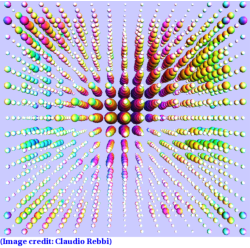
\includegraphics[width=0.5\textwidth]{figs/unit10_lattice.pdf}\end{center}

This approach of Wick rotating and then discretizing space and time is known as \textbf{lattice field theory}.
The image above comes from a lattice field theory computation that predicted properties of protons.
It visualizes a snapshot (at a single point in imaginary time) of the spatial configuration of a quark field within that proton.
Each quark degree of freedom has a ``color charge'' --- a linear combination of $\left\{\mbox{red}, \mbox{blue}, \mbox{green}\right\}$ --- whose orientation in colour space is indicated by the colour of each point in the illustration above, while the size of each points represents the magnitude of the charge.
By repeating these numerical calculations for discrete space-times with more lattice sites placed closer together, we can recover the original, continuous system by extrapolating to the  \textit{continuum limit} where there are infinitely many lattice sites infinitesimally close together.
Lattice field theory is an extremely successful and broadly applicable approach, which has proven able to predict many aspects of complicated interacting QFTs with high precision and controlled uncertainties that are systematically improvable through additional computing resources or algorithmic innovations.

\subsubsection*{Voter models}
Moving beyond the mathematical sciences, we can consider sociology as a domain where the applicability of statistical physics is less obvious.
Despite this, there is a diverse and active field of ``sociophysics'', which uses methods and perspectives of statistical physics to describe various aspects of social and political behaviour.
Serge Galam's 2012 book \href{https://liverpool.idm.oclc.org/login?url=http://dx.doi.org/10.1007/978-1-4614-2032-3}{\textit{Sociophysics}} provides a comprehensive introduction.
In the decade since it was published, the continued growth of enormous online social networks has unleashed a flood of data that can be modeled through frameworks based on interacting statistical systems.

A particular branch of sociology where connections to statistical physics may be more apparent is the field of opinion formation, where ``\href{https://en.wikipedia.org/wiki/Voter_model}{voter models}'' have been widely used since the 1970s to model elections, and more general political debates, with varying degrees of success.
Voter models are interacting statistical systems not too different from the Ising model, where the spin degrees of freedom that we have been working with are reinterpreted as voters' opinions on a certain topic.
For example, support for a particular proposition, individual candidate or political party can be represented as $s_n = +1$, with $s_n = -1$ indicating opposition.
Just like the interactions in the Ising model encourage spins to align with each other, voter models incorporate a tendency for voters to align (i.e., agree) with the majority of other voters they interact with.

There are many generalizations that can then be added to better describe the outcome of polls and elections.
A simple extension would be to allow voters to be neutral or indifferent to the question, represented as $s_n = 0$.
Similarly, the strength of a voter's commitment to their opinion can be modelled by extending the range of possible spin values,
\begin{equation*}
  s_n \in \left\{\cdots, -2, -1, 0, +1, +2, \cdots\right\}.
\end{equation*}

Voter models should also be defined on flexible and evolving \textit{graphs}, rather than the regular lattices we considered for the Ising model, in order to capture the possibility of people interacting with different sets of individuals over time.
The figure on the next page, from Richard Durrett et al., ``\href{https://doi.org/10.1073/pnas.1200709109}{Graph fission in an evolving voter model}'' (2012), illustrates how such a graph can look for a two-state voter model with $s_n \in \left\{-1, +1\right\}$ coloured red and blue.
As in everyday experience (and inspired by social networks), different voters have different numbers of connections with each other.
In this particular investigation, network connections between disagreeing voters are probabilistically severed, which enables a transition between two phases.
In one of these phases a consensus develops among the vast majority of voters.
In the other phase the population becomes increasingly polarized, as shown below.
Voters with a particular opinion increasingly interact only with others who share that opinion, and eventually nearly all connections are severed between the two opposing groups.

\begin{center}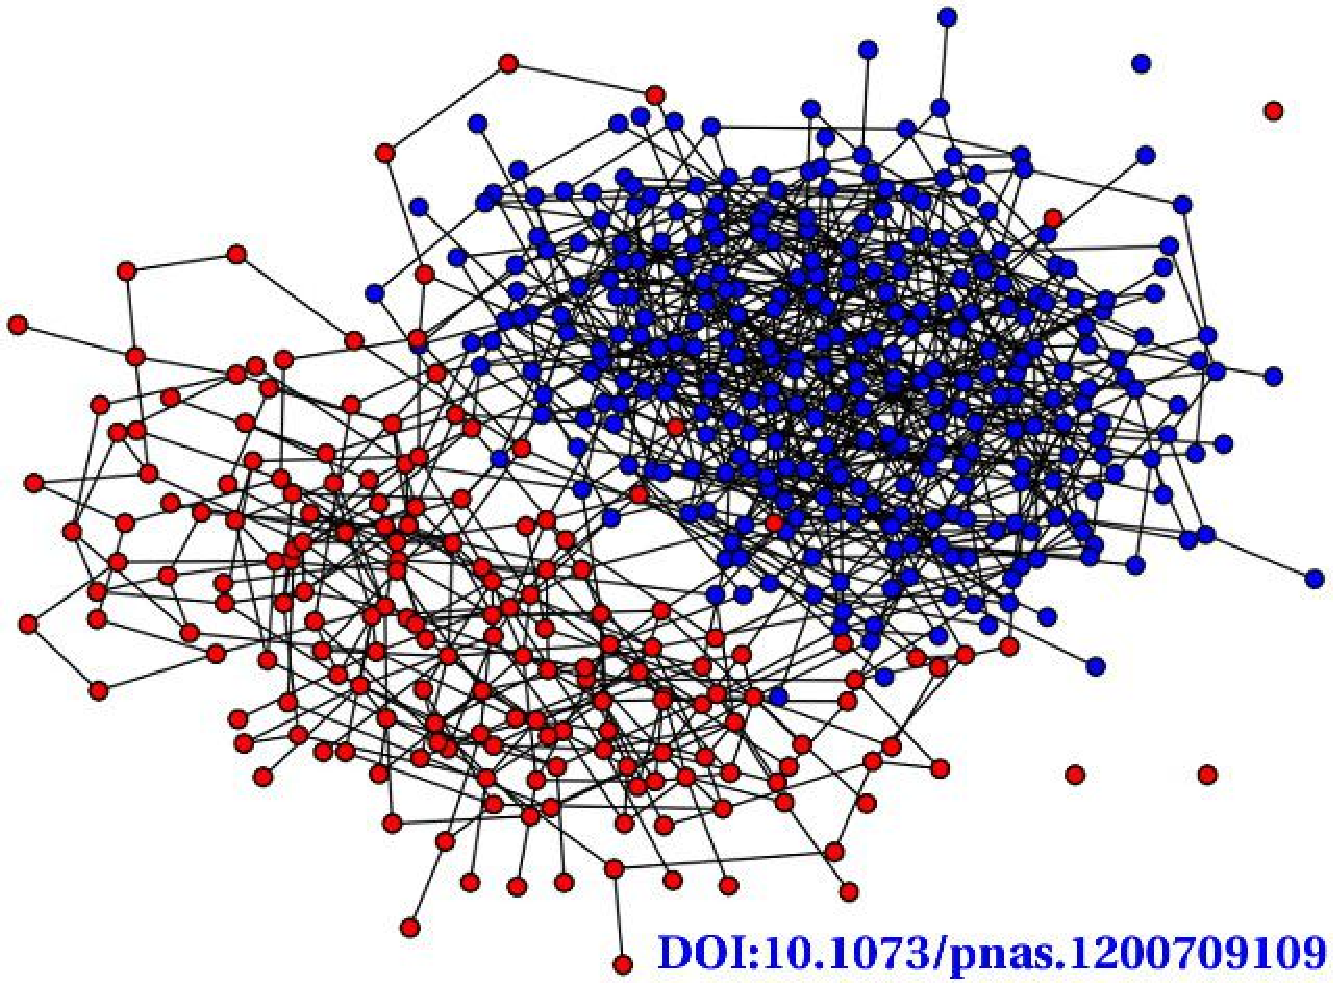
\includegraphics[width=0.7\textwidth]{figs/unit10_voter.pdf}\end{center}

Simpler studies, that don't allow connections to be severed, can also observe a transition to consensus once an opinion reaches a critical concentration.
In particular, Alexander Balankin et al., ``\href{https://doi.org/10.1016/j.physleta.2016.12.001}{Ising percolation in a three-state majority vote model}'' (2016) found this to be a second-order phase transition in the universality class of the two-dimensional Ising model.
This work also observed the possibility of a ``stable non-consensus'' phase, with long-term polarization between `clusters' of aligned voters who interact mainly with each other rather than with voters holding different opinions.
In this case, rather than severing connections between the two groups, the fixed patterns of connections encouraged voters to change their opinions until these stable clusters eventually formed.

\subsubsection*{Epidemiology}
Another application of interacting statistical systems, which has attracted a lot of attention in recent years, is to model the spread of diseases in populations.
As in the case of voter models, the degrees of freedom under consideration are again individuals, whose interactions with each other can allow the infection to spread to those who are susceptible.
Numerical Monte Carlo calculations can then be used to model how many people are likely to be infected as time passes, guided by data on typical movement and contacts.

The picture on the next page is a snapshot from \href{https://www.washingtonpost.com/graphics/2020/world/corona-simulator/}{an over-simplified simulation} provided by the \textit{Washington Post} to illustrate these concepts.
Here individuals are modeled simply as a gas of interacting particles in two dimensions, and various ways of restricting their motion are used to explore the likely effects of measures such as quarantines and social distancing.
By coincidence, the scale of this simulation, which considers a population of just $200$ people, is comparable to the first importance sampling Monte Carlo calculation carried out in 1953, which computed the pressure (i.e., equation of state) for $224$ interacting particles in a two-dimensional `volume'.
At the time, this required several days of computing time on a state-of-the-art machine; now these sorts of calculations are easily done on a smartphone.

\begin{center}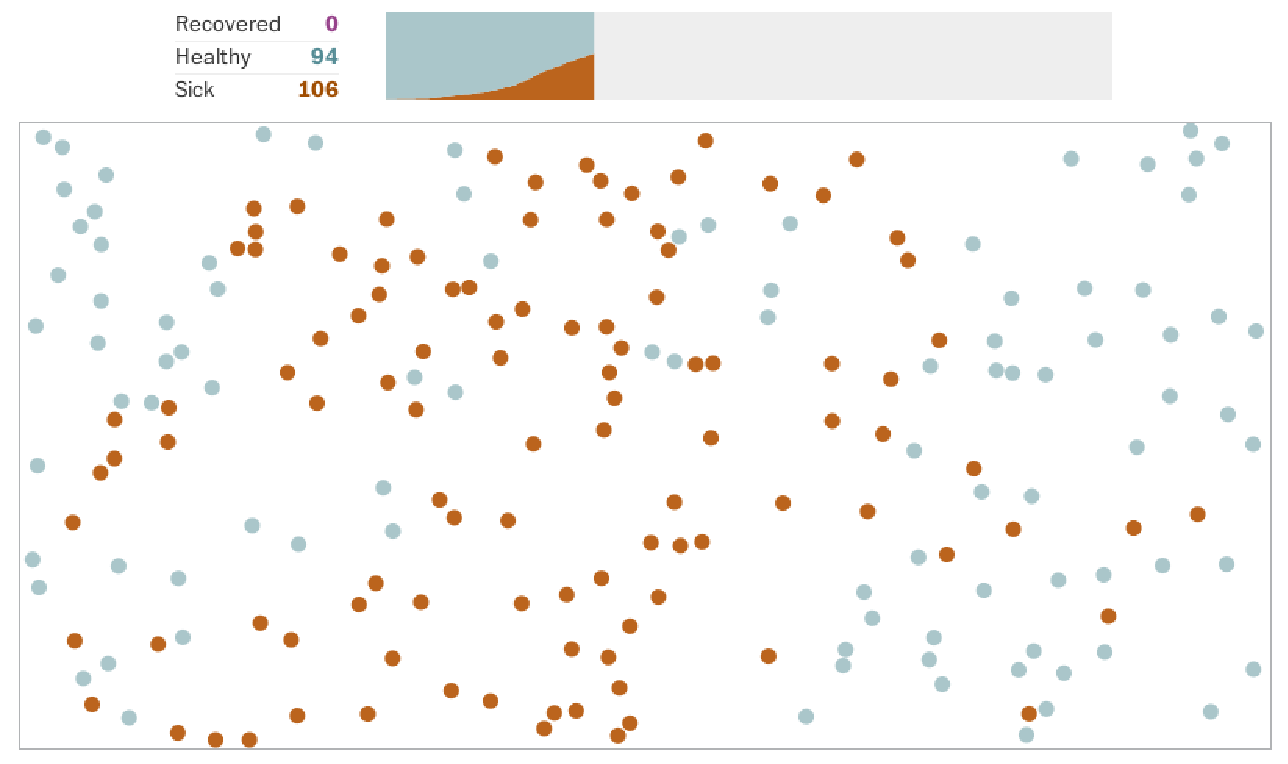
\includegraphics[width=0.8\textwidth]{figs/unit10_epidemic.pdf}\end{center}

Larger-scale and more realistic versions of these epidemiological simulations provide important input into government deliberations regarding what restrictions (such as lockdowns) would be most beneficial to reduce the spread of disease, and how long it would be best to maintain such restrictions.
Rather than investigating a phase transition, the goal is to quantify likely effects of various potential restrictions.
As described in \secref{sec:LLN}, the numerical experiments are therefore repeated many times with different sequences of pseudo-random numbers, to produce an ensemble of possibilities from which the likely outcomes of interventions can be inferred.

\subsubsection*{Flocking}
Let's conclude these brief highlights of some broader applications of statistical physics by considering another biological example, where interacting statistical systems are used to model the large-scale collective motion of certain groups of animals.
The image on the next page, from Marcus Woo, ``\href{https://www.sciencemag.org/news/2014/07/how-bird-flocks-are-liquid-helium}{How bird flocks are like liquid helium}'' (2014) illustrates the ``flocking'' behaviour of groups of starlings, which fly through the sky in surprisingly tight coordination, producing shape-shifting clouds known as \href{https://www.youtube.com/watch?v=V4f_1_r80RY}{murmurations}.
Qualitatively similar behaviour is also seen in schools of fish, swarms of insects, and even crowds of humans.

\begin{center}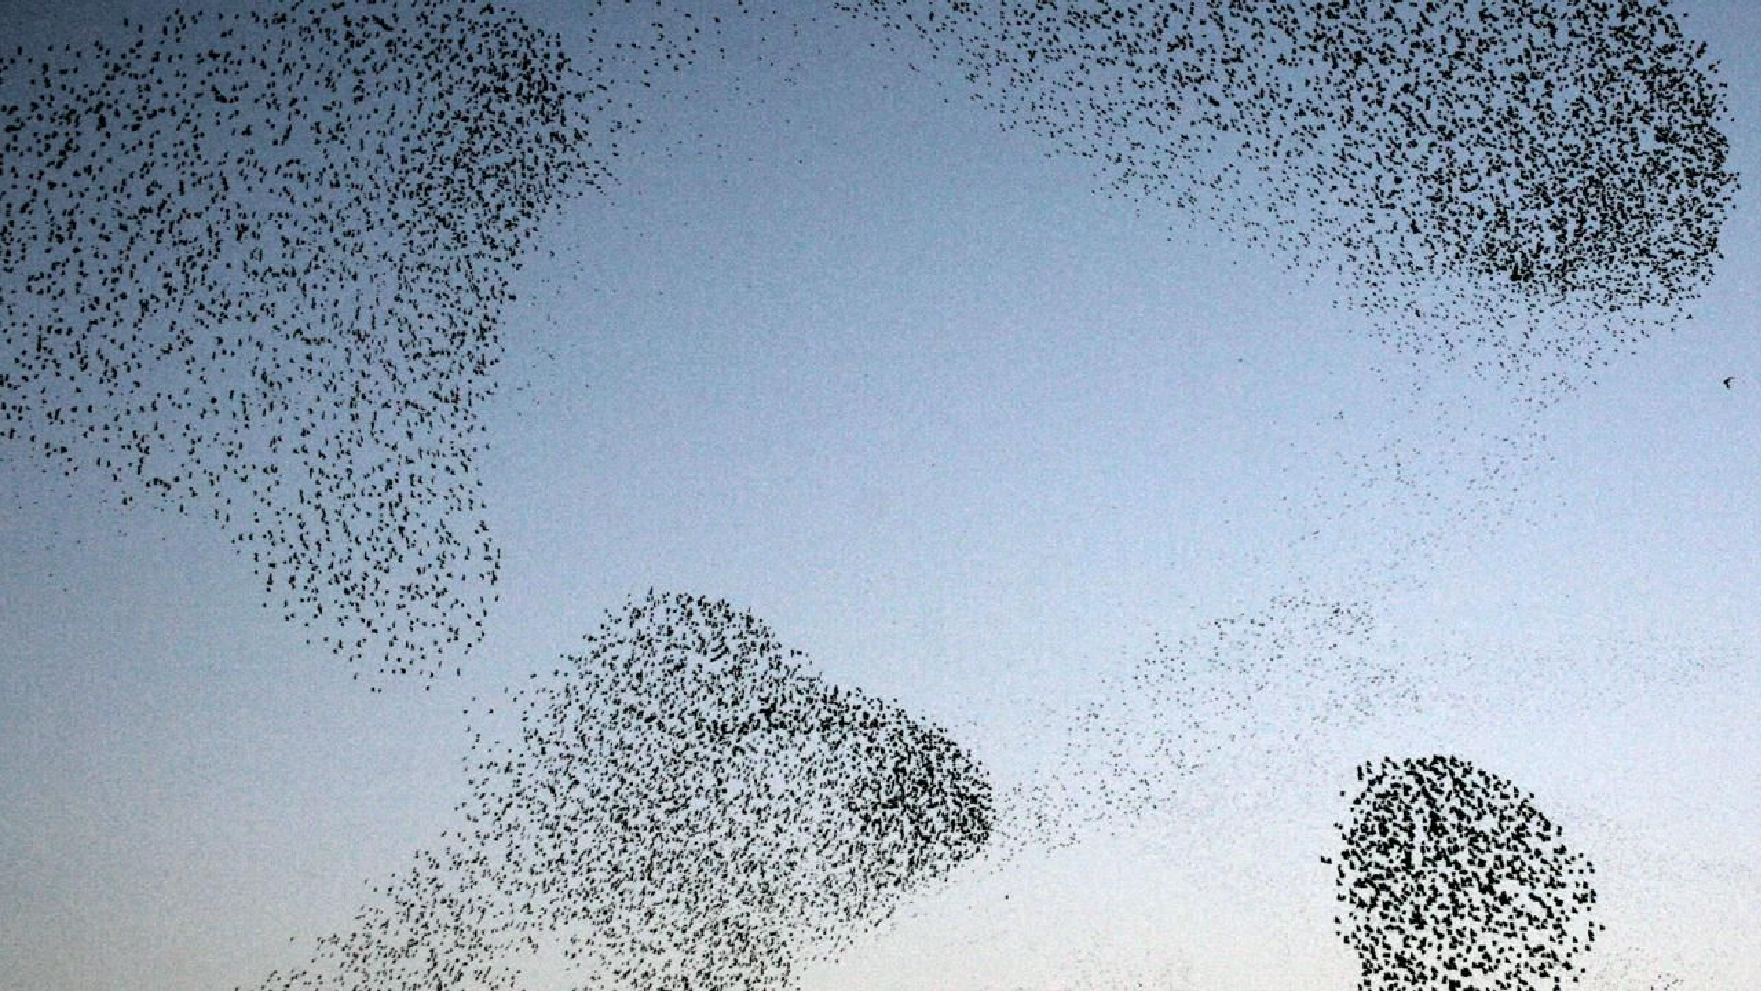
\includegraphics[width=0.8\textwidth]{figs/unit10_flock.pdf}\end{center}

Many models based on interacting statistical systems have been --- \href{https://doi.org/10.1038/s41467-022-29883-4}{and continue to be} --- developed to describe this emergent collective behaviour.
The recent work linked above builds upon a particularly simple ``\href{https://en.wikipedia.org/wiki/Vicsek_model}{Vicsek model}'' introduced in 1995, which hypothesizes that each particle (i.e., bird) will interact with others near to it.
These interactions encourage the particle to move in the same direction as its neighbours, similar to how the nearest-neighbour interactions in the Ising model encourage its spins to align.

Models of this sort exhibit a transition between two distinct phases.
When there is a low density of particles, there are relatively few interactions and the particles' motion is disordered, with no formation of murmurations or swarms.
At high densities, in contrast, large-scale collective motion appears, based solely on the interactions between the individual particles in the system.
An order parameter sensitive to this behaviour is the average angle of the particles' motion.
Different variations of the model can predict either a first-order or second-order transition between these two phases, and in the second-order case the universality class of the critical exponents can depend on the details of the variation. % doi.org/10.1140/epjb/e2008-00275-9
In some cases, as the critical density is approached from the disordered phase, the particles exhibit anomalous super-diffusion like that investigated in the computer project. % cond-mat/0401208
% ------------------------------------------------------------------



% ------------------------------------------------------------------
\subsection{Wrap-up recap and synthesis}
In this module we have built on foundations from probability theory to develop and apply the core concepts of statistical physics.
In Unit~1 we defined probability spaces, expectation values and variances, and used these to establish the law of large numbers through which stable large-scale behaviour occurs for stochastic systems that involve a large number of degrees of freedom, $N \gg 1$.
We also saw how the central limit theorem relates large-$N$ probability distributions to the underlying mean and variance of the elementary degree of freedom, and practiced extracting probabilities from such distributions.
The law of diffusion results from the central limit theorem, and the computer project applied inverse transform sampling to study how anomalous diffusion can arise when the central limit theorem's assumption of finite elementary mean and variance breaks down.

Starting in Unit~2 we specialized to focus on statistical ensembles in thermodynamic equilibrium as more specialized realizations of probability spaces.
These statistical ensembles consist of the set of micro-states $\om_i$ that a system can possibly adopt through its evolution in time, each with the corresponding probability $p_i$ that it will actually be adopted.
The laws of nature --- such as the first law of thermodynamics that requires conservation of energy --- impose constraints on statistical ensembles.
The micro-canonical ensemble directly implements such constraints, by requiring the system's internal energy and particle number be constant as it evolves in time, which means that the system must be completely isolated from the rest of the universe.
This makes both the entropy (\eq{eq:entropy}) and temperature (\eq{eq:temperature}) derived quantities, which we explored through the simple example of non-interacting spin systems.
In particular, we derived a form of the second law of thermodynamics, which states that the total entropy never decreases as time passes and therefore implies that maximal entropy corresponds to thermodynamic equilibrium.

Motivated by the impracticality of demanding that a system be completely isolated, in Unit~3 we turned to the canonical ensemble, which allows systems to exchange energy with a large thermal reservoir that imposes a constant temperature.
The particle number is still fixed, while the entropy, internal energy and heat capacity are now important derived quantities, with the last two related by a fluctuation--dissipation relation.
Maximizing the entropy to consider systems in thermodynamic equilibrium defines the partition function (\eq{eq:canon_part_func}) and Boltzmann distribution (\eq{eq:canon_prob}) as the fundamental mathematical definition of the system.
Derived quantities are determined from the partition function, or equivalently from the Helmholtz free energy (\eq{eq:helmholtz}).

By analyzing non-interacting systems of both distinguishable and indistinguishable spins, we demonstrated that the intrinsic information content of statistical systems has physically measurable effects.
These physical measurements are possible for canonical systems that don't have to be completely isolated, and in tutorials we saw that measured heat capacities for many materials can be modeled by the Einstein solid, with improved results obtainable through the Debye theory of solids.
These analyses highlighted the useful trick of considering high- and low-temperature limits in which statistical systems can simplify dramatically.

In Unit~4 we continued working with the canonical ensemble, applying it to study non-interacting (ideal) gases of non-relativistic, classical particles.
At the start of this analysis we had to regulate the system to ensure that its partition function was well-defined.
We did this by assuming that only discrete momenta are possible in a finite volume $V$, and then taking the limit of continuously varying momenta that allowed us to replace discrete sums with continuous integrals.
Considering ideal gases of both distinguishable and indistinguishable particles, we determined their partition functions and used these to derive the internal energy (\eq{eq:ideal_energy}) and entropy (\eq{eq:ideal_entropy}).
We saw that mixing two gases of distinguishable particles produces a positive mixing entropy, meaning that this process is irreversible, in contrast to combining and reseparating gases of indistinguishable particles.
Finally we defined the pressure as the change in the system's energy upon changing its volume while keeping its entropy constant (\eq{eq:pressure}), and derived the ideal gas law (\eq{eq:ideal_gas_law}) as a famous equation of state.

Building on these analyses of ideal gases in the canonical ensemble, in Unit~5 we considered thermodynamic cycles as systems that perform a repeatable sequence of expansions, compressions and heat transfers in order to act as heat engines or refrigerators.
This required first considering the work done on the system through these processes (\eq{eq:work}), the heat added to or removed from it (\eq{eq:heat_def}), and the first law of thermodynamics expressed in terms of these quantities (\eq{eq:first_law}).
As two limiting cases, we contrasted slow isothermal processes that feature sufficient heat exchange to keep the temperature constant, versus more realistic adiabatic processes that occur too quickly for any heat to be exchanged.
After introducing $PV$~diagrams as a convenient way to visualize thermodynamic cycles and the individual processes that comprise them, we analyzed the Carnot heat engine and computed how much work it can do on its surroundings as heat flows through it from a hot thermal reservoir to a cold reservoir.
This balance of work and heat defines the engine's efficiency (\eq{eq:efficiency}).
We showed that the Carnot cycle achieves the maximum possible efficiency allowed by the second law of thermodynamics, and in a tutorial we confirmed the lower efficiency of the Otto cycle that describes a petrol engine.

Returning to the formulation of statistical ensembles, in Unit~6 we further generalized our perspective to consider systems that can exchange both particles and energy with a large particle reservoir.
Introducing the chemical potential (\eq{eq:chem_pot}) as the new quantity that the particle reservoir keeps constant --- along with the temperature --- defined the grand-canonical ensemble.
A final round of entropy maximization gave us the grand-canonical partition function (\eq{eq:grand_part_func}) and the corresponding grand-canonical potential (\eq{eq:grand_pot}) that determine the derived quantities, which now include the particle number in addition to the internal energy and the entropy.
We were also able to derive a generalized thermodynamic identity (\eq{eq:thermo_ident}) that relates the chemical potential to the change in energy upon adiabatically adding a particle to the system.

Our main applications of the grand-canonical ensemble involved analyzing quantum gases, and as preparation for that we introduced quantum statistics in Unit~7 --- simply considering this as an ansatz rather than relying on prior knowledge of quantum mechanics.
After demonstrating how our earlier classical (non-quantum) approach to ideal gases breaks down when there is a non-negligible probability for multiple identical particles to occupy the same energy level, we got around this problem by organizing the micro-states in terms of the possible occupation numbers of the energy levels.
These possible occupation numbers distinguish between the two types of particles that appear in nature: bosons can have any non-negative occupation numbers $n_{\ell} \in \Nbb_0$, while fermions obey the Pauli exclusion principle and can have only $n_{\ell} \in \left\{0, 1\right\}$.
We derived (and factorized) the respective Bose--Einstein (\eq{eq:partfunc_BE}) and Fermi--Dirac (\eq{eq:partfunc_FD}) statistics for these two types of quantum particles, and checked that both approach classical Maxwell--Boltzmann statistics (\eq{eq:partfunc_MB}) in the limit of high temperature with large negative chemical potential $-\mu \gg T$.

With quantum statistics in hand, Unit~8 featured our analyses of quantum gases, first considering a non-interacting ideal gas of ultra-relativistic photons with energies defined in terms of frequencies (\eq{eq:photon_omega}).
Based on the grand-canonical potential, we derived the Planck spectrum (\eq{eq:Planck_omega}) governing the frequency dependence of the energy density for the photon gas, and found how it solves the ultraviolet catastrophe of the classical Rayleigh--Jeans spectrum.
We also saw how the Planck spectrum provides an excellent mathematical model for both solar radiation from stars --- among the hottest environments in the universe --- as well as the cosmic microwave background that fills frigid inter-galactic space and provides strong evidence for the existence of dark matter.
We finally derived the radiation pressure of photon gases, and the corresponding equation of state (\eq{eq:photon_eos}), which has the same form as the ideal gas law, just with a different numerical factor.

We continued with a similar application of the grand-canonical ensemble to ideal quantum gases of non-interacting fermions, focusing mainly on non-relativistic particles and considering the low-temperature regime where quantum Fermi--Dirac statistics differs the most from the classical case.
Again based on the grand-canonical potential, we derived the Fermi function $F(E)$ and saw how it approaches a step function at low temperatures.
This corresponds to all the low-lying energy levels being filled by the single fermion that can occupy each of them according to the Pauli exclusion principle.
The transition from filled to empty energy levels defines the Fermi energy, which in the zero-temperature limit is simply the chemical potential (\eq{eq:Fermi_energy}).
The resulting internal energy (\eq{eq:fermi_E_N}) and pressure (\eq{eq:degen_pressure}) remain positive even as the temperature approaches absolute zero.
This non-zero degeneracy pressure helps to explain the regularity of type-Ia supernovas, which play a key role in establishing the existence of so-called dark energy.
After more briefly deriving the equation of state for a relativistic ideal fermion gas, we wrapped up the non-interacting portion of the module by working through the Sommerfeld expansion that enabled us to predict the leading low-temperature corrections to the zero-temperature limits of $\frac{\mu}{E_F}$ (\eq{eq:mu_vs_T}) and the heat capacity ($c_v \propto T$).

Our final major topic was to explore the effects of interactions in statistical systems, making further use of the tools we had previously developed.
Statistical systems in which the constituent degrees of freedom interact with each other can exhibit a broader array of phenomena, such as phase transitions.
At the same time, they become enormously more difficult to analyze, because their partition functions and derived quantities no longer factorize into independent single-particle contributions.
In Unit~9 we focused on the famous Ising model, which is simple to write down as a system of spins interacting with their nearest neighbours on a $d$-dimensional lattice (\eq{eq:Ising_energy}), but extremely difficult to solve exactly in two or more dimensions.
For $d \geq 2$ dimensions, the Ising model exhibits a second-order phase transition between its high-temperature disordered phase and its low-temperature ordered phase, with its magnetization serving as the order parameter.
We analyzed the Ising model through the mean-field approximation that produced a self-consistency condition (\eq{eq:consistency}) for its order parameter, the magnetization.
We then exactly solved the one-dimensional Ising model and used Kramers--Wannier duality to predict the exact critical temperature in two dimensions, showing that the mean-field approximation is not very reliable in a low number of dimensions.

Although the mean-field approximation to the Ising model does capture a second-order phase transition, the critical temperature and critical exponents it predicts for this transition only slowly converge towards the correct values as the dimensionality of the system increases.
Determining the correct critical behavior in $d > 2$ dimensions requires numerical analyses that we discussed in this final Unit~10.
Monte Carlo importance sampling algorithms are the standard way to carry out reliable numerical computations with controlled uncertainties in a realistic amount of time, and are very broadly applicable to more general interacting statistical systems.
Amazingly, extremely different physical systems can exhibit transitions characterized by exactly the same critical exponents, a phenomenon known as universality, which helps to explain the broad applicability and far-reaching power of statistical physics.

In summary, we have learned foundations including statistical ensembles, entropy, and the laws of thermodynamics.
We have studied applications including diffusion, ideal gases, thermodynamic cycles, and phase transitions.
And we have explored advanced topics including numerical methods and universality.
All together, our new knowledge of statistical physics enables us to observe and appreciate many further applications of these concepts and tools across the mathematical sciences and beyond.
% ------------------------------------------------------------------
